\documentclass[a4paper,14pt]{extarticle}
\usepackage[utf8]{inputenc}
\usepackage[russian]{babel}
\usepackage{graphicx}
\usepackage{indentfirst}
\usepackage[top=0.8in, bottom=0.8in, left=0.8in, right=0.8in]{geometry}
\usepackage{pgfplots}
\usepackage{amsmath}
\usepackage{setspace}
\usepackage{titlesec}
\usepackage{pdfpages}
\usepackage{subcaption}
\usepackage{float}
\usepackage{longtable}
\usepackage{chngcntr}
\usepackage{pgfplots}
\usepackage{amsfonts}
\usepackage{hhline}
\usepackage{pgfplotstable}
\usepackage{multirow}
\usepackage{tikz,xcolor}
\usepackage{listings}

\lstset{ %
extendedchars=\true,
keepspaces=true,
language={[x86masm]Assembler},					% choose the language of the code
basicstyle=\footnotesize,		% the size of the fonts that are used for the code
numbers=left,					% where to put the line-numbers
numberstyle=\footnotesize,		% the size of the fonts that are used for the line-numbers
stepnumber=1,					% the step between two line-numbers. If it is 1 each line will be numbered
numbersep=10pt,					% how far the line-numbers are from the code
backgroundcolor=\color{white},	% choose the background color. You must add \usepackage{color}
showspaces=false, 			% show spaces adding particular underscores
showstringspaces=false,			% underline spaces within strings
showtabs=false,					% show tabs within strings adding particular underscores
frame=single,           		% adds a frame around the code
tabsize=4,						% sets default tabsize to 2 spaces
captionpos=b,					% sets the caption-position to bottom
breaklines=true,				% sets automatic line breaking
breakatwhitespace=false,		% sets if automatic breaks should only happen at whitespace
escapeinside={\%*}{*)},			% if you want to add a comment within your code
%postbreak=\raisebox{0ex}[0ex][0ex]{\ensuremath{\color{red}\hookrightarrow\space}}
}

\titleformat{\section}[hang]
  {\bfseries}
  {}
  {0em}
  {\hspace{-0.4pt}\large \thesection\hspace{0.6em}}
  
  
\titleformat{\subsection}[hang]
  {\bfseries}
  {}
  {0em}
  {\hspace{-0.4pt}\large \thesubsection\hspace{0.6em}}
  
\titleformat{\subsubsection}[hang]
  {\bfseries}
  {}
  {0em}
  {\hspace{-0.4pt}\large \thesubsubsection\hspace{0.6em}}

%\linespread{1.3} % полуторный интервал
%\renewcommand{\rmdefault}{ftm} % Times New Roman

\counterwithin{figure}{section}
\counterwithin{equation}{section}
\counterwithin{table}{section}

\begin{document}
\begin{titlepage}
\centering
Санкт-Петербургский политехнический университет Петра Великого \\
Институт компьютерных наук и технологий \\
Кафедра компьютерных систем и программных технологий \\
\vspace{5.5cm}

{\centering \textbf{Отчёт по лабораторной работе} \\ 
\vspace{0.15cm}
\textbf{Дисциплина}: Технологии компьютерных сетей \\
\vspace{0.15cm}
\textbf{Тема}: Программирование сокетов протоколов TCP и UDP } \\

\vspace{5.5cm}

\begin{table}[H]
\begin{tabular}{p{\textwidth}@{}r}
{Выполнили студенты гр. 43501/3} \hfill 
\vspace{0.2cm}
Мальцев М.С. \\ \hfill
\vspace{0.2cm}

Преподаватель \hfill 
\vspace{0.2cm}
Зозуля А.В \\ \hfill 
\vspace{0.2cm}

{} \hfill { <<\underline{\hspace{0.08\textwidth}}>> \underline{\hspace{0.2\textwidth}}2018 г.} \\
\end{tabular}
\end{table}
\vfill
{\centering Санкт-Петербург \\ 
\vspace{0.15cm}
2018}
\end{titlepage}

\section{Цель работы.}
Ознакомиться с принципами работы протоколам TCP и UDP.

\section{Задание}
\textbf{Система распределенных математических расчетов}

Разработать распределенную систему, состоящую из приложений клиента и сервера, для распределенного расчета простых чисел.
Информационная система должна обеспечивать параллельную работу нескольких клиентов.

\textbf{Серверное} приложение должно реализовывать следующие функции:
\begin{enumerate}
\item Прослушивание определенного порта
\item  Обработка запросов на подключение по этому порту клиентов
\item Поддержка одновременной работы нескольких клиентов с использо-
ванием механизма нитей и средств синхронизации доступа к разде-
ляемым между нитями ресурсам.
\item Принудительное отключение конкретного клиента
\item Хранение рассчитанных клиентами простых чисел, а также текущей
нижней границы диапазона для нового запроса на расчет
\item  Выдача клиентам максимального рассчитанного простого числа
\item Выдача клиентам последних N рассчитанных простых чисел
\item Выдача клиентам необходимого диапазона расчета чисел
\item Сохранение состояния при выключении сервера
\end{enumerate}

\textbf{Клиентское} приложение должно реализовывать следующие функции:
\begin{enumerate}
\item Возможность параллельной работы нескольких клиентов с одного
или нескольких IP-адресов
\item Установление соединения с сервером (возможно, с регистрацией на
сервере)
\item Разрыв соединения
\item Обработка ситуации отключения сервером
\item Получение от сервера и вывод максимально рассчитанного простого
числа
\item Получение от сервера и вывод последних N рассчитанных простых
чисел
\item Получение от сервера диапазона расчета простых чисел (нижнюю
грань выдает сервер, количество проверяемых чисел - клиент)
\item Расчет простых чисел в требуемом диапазоне (имеет смысл прове-
рять остатки от деления на все нечетные числа в пределах
sqrt(Nmax)+1)
\item Передача серверу набора рассчитанных простых чисел
\end{enumerate}

\section{Ход работы}
\subsection{Прикладной протокол}
Для решения поставленной задачи был разработан прикладной протокол передчаи данных. Планируемая длина пакета в протоколе равна 26 байт.

\textbf{Запросы} :
\begin{itemize}
\item	MAX -- Выдача максимального рассчитанного простого числа

	[MAX]?;


\item	LAST [number] -- Выдача последних N рассчитанных простых чисел

	[LAST]?[number];


\item	FROM -- Выдача диапазона для расчета чисел

	[FROM]?;

	
\item	POST [number] -- Загрузка на сервер расчитаного числа

	[POST]?[number];

\end{itemize}

\textbf{Ответы} :
\begin{itemize}
\item	200;  - OK [data]

\item	400; - Bad Request
\end{itemize}

\subsection{Описание архитектуры}
Архитектура серверного приложения изображена на UML диаграме, рисунок \ref{uml-1}.
\begin{figure}[H]
	\begin{center}
		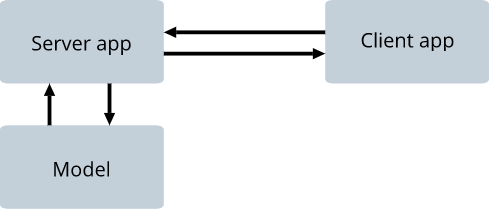
\includegraphics[scale=0.6]{pics/1}
		\caption{UML-диаграмма компонентов приложения}
		\label{uml-1}
	\end{center}
\end{figure}

Разработаная архитекутра использовалась как для создания UDP, так и для создания TCP приложения.
Причём, при реализации TCP и UDP приложений, компонент под названием $Model$, который отвечает за бизнес логику оставался неизменным.
Также для обоих приложений общими стали файл, отвечающий за конфигурацию серверной части приложения и файл, содержажщий небольшие функции, типа разделения строки по символу.

\subsubsection{Бизнес логика}
Основная задача этого компонента -- это предоставление функций:
\begin{itemize}
\item хранения и выдача по запросу уже существующих чисел
\item сохранение новых чисел
\item проверка дублирования чисел
\item выдача новых диапазонов для расчета простых чисел
\item в случае, если диапазон был запрошен, но данные по нему не пришли в течении некоторого времени, то диапазон снова помещается в пул выдаваемых
\end{itemize}

Для этого компонента был разработан следующий интерфейс представленный на рисунке \ref{SimpleNumbers}.
\begin{figure}[H]
	\begin{center}
		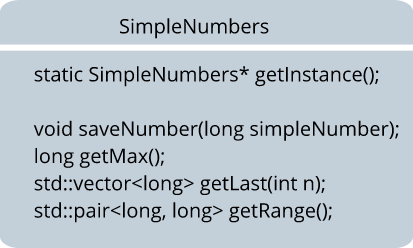
\includegraphics[scale=0.5]{pics/SimpleNumbers}
		\caption{Интерфейс компонента, отвечающего за бизнес логику}
		\label{SimpleNumbers}
	\end{center}
\end{figure}

Был применен шаблон проектирования Singleton. Это было продиктовано тем, что подобный компонент в системе должнен быть только однин.


\subsubsection{TCP сервер и клиент}
Архитектура серверной части TCP приложения представлена на рисунке \ref{serverTCP}.
\begin{figure}[H]
	\begin{center}
		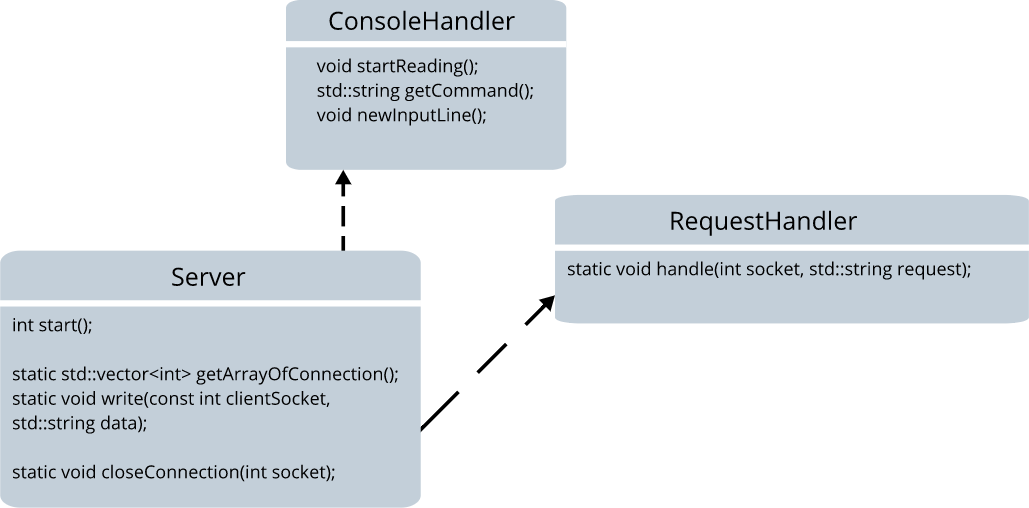
\includegraphics[scale=0.4]{pics/serverTCP}
		\caption{UML-диаграмма классов TCP сервера}
		\label{serverTCP}
	\end{center}
\end{figure}

\textbf{ConsoleHandler} -- класс, отвечающий за считываение и обработку консольных команд. Запускается в отдельном процессе.

\textbf{RequsetHandler} -- класс, отвечающий за обработку запросов и генерацию ответов.

\textbf{Server} -- основной класс, задача которого принять и обработать входящее соединение и вызвать соответствующий обработчик. Также запускает ConsoleHandler в отдельном процессе.\\

Интерфейс клиентской части TCP приложения представлена на рисунке \ref{clientTCP}.
\begin{figure}[H]
	\begin{center}
		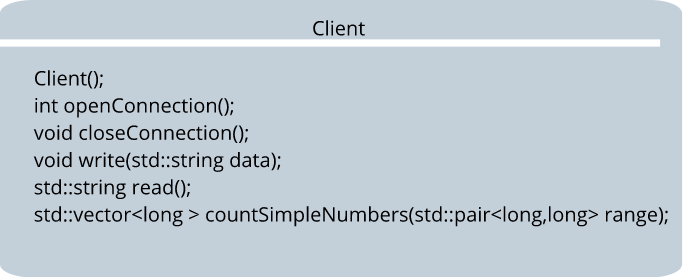
\includegraphics[scale=0.4]{pics/clientTCP}
		\caption{Интерфейс TCP клиента}
		\label{clientTCP}
	\end{center}
\end{figure}

Поверх этого класса, обеспечивающего работу с TCP сервером было разработано консольное приложение, которое принимало и выполняло команды пользователя.

Описание интерфеса:
\begin{itemize}
\item $next$ -- получить диапазон от сервера, вычислить все простые числа на нем и отправить их на сервер
\item $max$ -- запросить максимальное вычисленное простое число
\item $last [number]$ -- запросить $number$ последних простых чисел
\item $exit$ -- закончить обмен и закрыть соединение
\end{itemize}

\subsubsection{UDP сервер и клиент}
Общая идея работы серверного и клиентского UDP приложения  похожа на работу TCP приложения. Основные отличия заключаются в том, что при использовании UDP структура пакета урпощается и вопросы надженой передачи данных решаются разработчиком на прикладном уровне.

В описаном задании требуется обеспечить надженость работы приложения путем разрешения трех проблемных моментов:
\begin{itemize}
\item Потеря пакетов
\item Дублирование пакетов
\item Перемешивание пакетов
\end{itemize}

В данной реализации эти вопросы решаются следующим способом. Проблема потери пакетов решается использованием подтверждающих пакетов, иначе называемых как Acknowledgement или ACK. Проблема дубилрования исчезает в связи с тем, что если на клиентскую часть приходит несколько ответов, то ничего плохого в этом нет, а если на серверную, то она способна грамотно обработать, если это действительно критично. Например, если приходит несколько запросов POST с одинаковым число, то сервер запишет лишь одно, а если несколько запросов на рассчитываемый интервал, то он их выдаст, но когда через некторое время поймет, что ему никто не отвечает на них, отзовет интервалы обратно. Случай с перемешиванием пакетов тоже не является критичным в связи с тем, что посылаемые запросы довольно просты и не требуют определенной последовательности. Они могут одинаково успешно обрабатываться в любой последовательности.

Также небольшие изменения в проекте вызвал и тот факт, что пришлось изменять сигнатуры функций, потому что для идентификация UDP клиента со стороны сервера используются структуры данных, вместо переменной типа integer, как это было в TCP.

\subsection{Результаты тестирования}

Приложения были протестированы и продемонстрированы преподавателю. Тестирование проводилось в следующих условиях:
\begin{itemize}
\item 10 клиентов одновременно отправляли всевозможноые запросы на сервер, причем переодически старые заврешали работу и запускались новые
\item некоторые соединения намеренно обрывались, с целью проверить корректность обработки данных ситуаций
\item при завершении работы сервера проверялось, что все клиентские приложения получили уведомления о корректном окончании передачи данных
\item отдельно для UDP были промоделированы три проблемные ситуации (потеря, дублирование, перемешивание пакетов)
\end{itemize}
Разработанные приложения как TCP, так и UDP успешно справились с тестированием. Во всех перечисленных случаях система уверенно выполняла предписанные требования и справлялась со своей основной задачей -- распределенным вычислением простых чисел.

\section{Вывод}
В результате выполнения работы было разработано два приложения отличающиеся протоколом передачи данных, который они использовали. Оба приложения успешно выполняли свою основную задачу -- распределенное вычисление простых чисел. Было улучшено понимание принципов работы протоколов TCP и UDP.

К особенностям TCP можно отнести то, что соединение между клиентом и сервером является надёжным. Гарантируется доставка и правильная очередность пакетов. Что облегчает разработку приложения, к минусам же можно отнести меньшую скорость работы по сравнению с UDP.

К особенностям UDP можно отнести предельную простоту передающегося пакета, что обеспечивает высокую скорость передачи данных. Но в тоже время появляются проблемы надежности передачи. Пакет может не дойти до получателя, может быть отправлен несколько раз, также пакеты могут прйти в случайной последовательности. Все это осложняет разработку UDP приложения. Также к особенностям можно отнести то, что, в отличие от TCP, при использовании UDP четкого разделения между серверной частью приложения и клиентской нет. Это можно понять лишь анализируя трафик.

Исходя из полученного опыта, можно сделать вывод, что в случае, когда есть возможность использовать TCP, надо это делать. Но бывает, что очень критична скороcть передачи и не так критична надежность, к примеру при передче видео, или устройству не хватает вычислительность мощности для своевременной обработки структуры пакета TCP, в этом случае стоит использовать UDP.

Исходный код разработанного приложения размещен в git-репозитории $https://github.com/mikle9997/networks\_and\_telecommunications$

\section{Приложение 1. Листинги исходного кода. }
\lstinputlisting{../tcp/Config.h}

\lstinputlisting{../tcp/Config.cpp}

\lstinputlisting{../tcp/Utility.h}

\lstinputlisting{../tcp/Utility.cpp}

\lstinputlisting{../tcp/server/ConsoleHandler.cpp}

\lstinputlisting{../tcp/server/ConsoleHandler.h}

\lstinputlisting{../tcp/server/main.cpp}

\lstinputlisting{../tcp/server/RequestHandler.h}

\lstinputlisting{../tcp/server/RequestHandler.cpp}

\lstinputlisting{../tcp/server/Server.cpp}

\lstinputlisting{../tcp/server/Server.h}

\lstinputlisting{../tcp/server/model/FileStorage.cpp}

\lstinputlisting{../tcp/server/model/FileStorage.h}

\lstinputlisting{../tcp/server/model/SimpleNumbers.h}

\lstinputlisting{../tcp/server/model/SimpleNumbers.cpp}

\lstinputlisting{../udp/Config.h}

\lstinputlisting{../udp/Config.cpp}

\lstinputlisting{../udp/Utility.h}

\lstinputlisting{../udp/Utility.cpp}

\lstinputlisting{../udp/server/main.cpp}

\lstinputlisting{../udp/server/RequestHandler.h}

\lstinputlisting{../udp/server/RequestHandler.cpp}

\lstinputlisting{../udp/server/Server.cpp}

\lstinputlisting{../udp/server/Server.h}

\lstinputlisting{../udp/server/model/FileStorage.cpp}

\lstinputlisting{../udp/server/model/FileStorage.h}

\lstinputlisting{../udp/server/model/SimpleNumbers.h}

\lstinputlisting{../udp/server/model/SimpleNumbers.cpp}

\end{document}
